\ifx\allfiles\undefined
\documentclass{article}
\usepackage{graphicx}
\usepackage{float}
\usepackage{geometry}
\usepackage{hyperref}
\usepackage{amssymb}
\usepackage{booktabs}
\usepackage{tabularx}
\usepackage{amsthm}
\usepackage{amsmath}
\usepackage{enumitem}
\usepackage{tikz}
\usetikzlibrary{shapes.geometric, automata, positioning, arrows, calc, arrows.meta}

\geometry{left=1.2in, right=1.2in, top=1.5in, bottom=1.5in}
\linespread{1.5}%行距

% 设置列表环境的上下间距
\setenumerate[1]{itemsep=5pt,partopsep=0pt,parsep=\parskip,topsep=5pt}
\setitemize[1]{itemsep=5pt,partopsep=0pt,parsep=\parskip,topsep=5pt}
\setdescription{itemsep=5pt,partopsep=0pt,parsep=\parskip,topsep=5pt}

\theoremstyle{definition}
\newtheorem{defn}{\textbf{\textit{def}}}[section]
\newtheorem{prop}{\textbf{\textit{prop}}}[section]
\newtheorem{thm}[defn]{\textbf{\textit{thm}}}
\newtheorem{corollary}[defn]{\textbf{\textit{corollary}}}
\newtheorem{lemma}[defn]{\textbf{\textit{lemma}}}
\newtheorem{criterion}[defn]{\textbf{\textit{criterion}}}
\newtheorem{claim}[defn]{\textbf{\textit{claim}}}

\newtheorem{example}{\textbf{\textit{e.g.}}}[section]
\newtheorem{exercises}{\textbf{\textit{exercises}}}[section]
\newtheorem*{remark}{\textbf{\textit{remark}}}

\newenvironment{solution}{\par{\textit{solution}}\;}{\qed\par}

\def\R{\mathbb{R}} % 实数域
\def\N{\mathbb{N}} % 自然数域
\def\Q{\mathbb{Q}} % 有理数域
\def\Z{\mathbb{Z}} % 整数域
\def\eps{\varepsilon} %ε

\def\bgtbl{\begin{table}[htbp]
    \centering
    \begin{tabularx}{\textwidth}{XXXXX}}
\def\bgpic{\begin{tikzpicture}[->,>=stealth',shorten >=1pt,auto,node distance=2.5cm,semithick]
    \tikzstyle{every state}=[fill=white,draw=black,text=black]}
\graphicspath{{pictures/},{../pictures/}}  % 配置图形文件检索目录
\begin{document}
\else
\fi
\newpage
\section{Introduction}
\subsection{Big-O Notation}

\begin{defn}
    \textit{Let $f,g:\N \rightarrow \R$}
    \begin{itemize}
        \item \textit{Write $f = O(g)$ if $(\exists c > 0)(\exists N)(\forall n \geq N)(|f(n)| \leq cg(n))$.}
        \item \textit{Write $f = \Omega(g)$ if $(\exists c > 0)(\exists N)(\forall n \geq N)(|f(n)| \geq cg(n))$.}
        \item \textit{Write $f = \Theta(g)$ if $(\exists c_1, c_2 > 0)(\exists N)(\forall n \geq N)(c_1g(n) \leq |f(n)| \leq c_2g(n))$.}
        \item \textit{Write $f = o(g)$ if $(\forall \epsilon > 0)(\exists N)(\forall n \geq N)(|f(n)| \leq \epsilon g(n))$.}
    \end{itemize}

    Big-O Notation is the most commonly used one among the four.
\end{defn}


\begin{example}
    $f(n) = 6n^4-3n^3+5 \Rightarrow f(n) = O(n^4)$
\end{example}

\begin{proof}
    $|6n^4-3n^3+5|\leq 6n^4+3n^4+5n^4=13n^4$
\end{proof}


\begin{example}
    $\sum\limits_{i=1}^{n} i^2=\frac{n(n+1)(2n+1)}{6} = O(n^3)$
\end{example}
  
\begin{exercises}
    \textit{Write in big-O notation:}
    \begin{enumerate}
        \item $5 + 0.001n^3 + 0.25n$
        \item $500n+100n^{1.5}+50n\log_{10} n$
        \item $n^2\log_{2} n+n(\log_{2} n)^2$
        \item $3\log_{8}n+\log_2(\log_2 n)$
    \end{enumerate}
    \begin{solution}
        $O(n^3);O(n^1.5);O(n^2\log n);O(\log n)$
    \end{solution}
\end{exercises}
\begin{prop}\
    \begin{itemize}
        \item $f_1 = O(g_1),f_2=O(g_2)\Rightarrow f_1f_2=O(g_1g_2)$
        \item $f(O(g))=O(fg)$
        \item $f_1 = O(g_1), f_2 = O(g_2) \Rightarrow f_1 + f_2 = O(max(g_1, g_2))$
        \item $f_1 = O(g), f_2 = O(g) \Rightarrow f_1 + f_2 = O(g)$
        \item $f = O(g)\Rightarrow kf = O(g)$
    \end{itemize}
    \textbf{\indent often encountered:}
    \begin{itemize}
        \item \textit{constant: $O(1)$}
        \begin{itemize}
            \item $\sum\limits_{k=1}^{n}\frac{1}{k} = \ln n+O(1)$
            \item $\sum\limits_{k=1}^{n}\frac{1}{k^2} = O(1)$
            \item $\sum\limits_{k=1}^{n}\frac{1}{k\ln k} = \ln \ln n + O(1)$
        \end{itemize}
        \item \textit{double logarithmic: $O(\log \log n)$}
        \item \textit{logarithmic: $O(\log n)$}
        \item \textit{polylogarithmic: $O((\log n)^c), c > 0$}
        \item \textit{linear: $O(n)$}
        \item \textit{quasilinear: $O(n\log ^c n),O(n\log^{O(1)}n)$}
        \item \textit{quadratic: $O(n^2)$}
    \end{itemize}
\end{prop}

\begin{defn}
    $\omega(g),\theta(g)$
    \begin{itemize}
        \item $f=\omega(g)$ $if(\forall c>0)(\exists N)(\forall n\geq N)(f(n)\geq cg(n))$
        \item $g=\theta(g) ~(or ~ equivalently ~ f \sim g) ~ if ~ (\forall \epsilon > 0)(\exists N)(\forall n \geq N)(|f(n) - g(n)| < \epsilon g(n))$
    \end{itemize}
\end{defn}
\subsection{Alphabets and Languages}
\begin{defn}
    $(alphabet)~ An ~ alphabet ~ is ~ a ~set ~ of ~ symbols$
    \begin{itemize}
        \item $Roman~alphabet:a,b,c,d,\cdots,z$
        \item $binary~alphabet:0,1$
    \end{itemize}
\end{defn}
\begin{defn}
    \textit{(string and its length)}

    \textit{A \textbf{string} (over an alphabet) is a finite sequence of symbols from the alphabet.\\ \textbf{Empty string} is string of no symbols, denoted by $\varepsilon$.}
    
    \textit{The set of all string is denoted by $\Sigma ^ *$. Denote by $\Sigma^n$ the set of all \textbf{string of length} n. \\So, $\Sigma^* = \cup_{n\geq 0}\Sigma^n$.}

    \textit{Denote the length of a string w by $|w|$}
\end{defn}

\begin{example}
    $\{0,1\}^*=\{\varepsilon,0,1,00,01,\cdots\},|\varepsilon|=0,|0110|=4$    
\end{example}

\begin{defn}
    \textit{(concatenation) Two strings over the same alphabet can be combined by the operation of \textbf{concatenation}. The concatenation of x and y is denoted by xy.}
\end{defn}

\begin{defn}
    \textit{(substring, suffix, prefix) \\A string v is a substring of w if $\exists$ strings x and y such that w = xvy.\\ \indent If w = xv for some x, then v is a \textbf{suffix} of w.\\ \indent If w = vy for some y, then v is a \textbf{prefix} of w.}
\end{defn}

\begin{defn}
    \textit{("power") The string $w^i$ is defined: $w^0 = \varepsilon,w^{i+1}=w^iw,i \in \N$}
\end{defn}
\begin{example}
    $01^0 = \eps, 01^1 = 01, 01^2 = 0101$
\end{example}
\begin{defn}
    \textit{(reversal) The reversal of a string w,denoted by $w^R$,is the string "spelled backwards"}

    \textit{A formal definition can be given by induction on length:}

    \begin{enumerate}
        \item \textit{If $w = \eps,w^R = w = \eps$}
        \item \textit{If $|w| = n+1$,where $w = ua,a\in \Sigma$,then $w^R = au^R$}
    \end{enumerate}
\end{defn}

\begin{defn}
    \textit{(language) \textbf{Language} is a set of strings over an alphabet, That is, $L\subseteq \Sigma^*$.\\ \indent For example,$\emptyset,\Sigma^*,\Sigma$ are all languages}
    \begin{itemize}
        \item $\sigma = \{0,1\}$
        \item $Even = \{0,10,100,110,\cdots,\}$
        \item $Odd = \{1,11,101,\cdots\}$
        \item $Prime = \{10,11,101,111,\cdots\}$
        \item $Palindrome = \{w|w^R=w\}=\{\eps,0,1,00,11,\cdots\}$
    \end{itemize}
\end{defn}

\begin{defn}
    \textit{(complement, binary language operations)}

    \textit{Let L be a language. The \textbf{complement} of L, denoted by $\overline{L}$, is $\Sigma^*-\overline{L}$. So $\overline {\overline{L}}= L$.}

    \textit{Note that since L is a set, we can define \textbf{union}($\cup$), \textbf{interchapter*}($\cap$) and difference.}

    \textit{The \textbf{concatenation} of $L_1$ and $L_2$ is defined by $L_1L_2 = {w \in \Sigma^*, w = xy, \exists x \in L_1, y \in L_2}$}
\end{defn}

\subsection{Encoding of Problems}

\subsubsection{Examples}

\begin{enumerate}
    \item \textit{(\textbf{Integer multiplication}) Given two non-negative integers x, y, compute xy.}
    \item \textit{(\textbf{Primality testing}) Given $n \in \N$, decide if n is a prime.}
    \item \textit{(\textbf{Hamiltonian cycle}) Given an undirected graph G, test if G has a Hamiltonian cycle.}
\end{enumerate}

\subsubsection{Analysis}

\begin{itemize}
    \item \textit{\textbf{Decision} problem: 2,3}
    \item \textit{\textbf{Computation} problem: 1}
\end{itemize}

\subsubsection{Conclusion}
\begin{itemize}
    \item \textit{By \textbf{encoding}, decision problem is language. Any computation problem is a function from $\Sigma^*$ to $\Sigma^*$. Our course only concerns decision problem, namely language.}
    \item \textit{By \textbf{preprocessing}, one can switch between encodings.}
\end{itemize}

\begin{example}
    \
    \begin{itemize}
        \item \textit{graph}

        \begin{tikzpicture}
            % Define nodes
            \node[circle,draw] (A) at (0,-1) {A};
            \node[circle,draw] (B) at (2,0) {B};
            \node[circle,draw] (C) at (4,-1.) {C};
            
            % Draw edges
            \draw (A) -- (B);
            \draw (B) -- (C);
        \end{tikzpicture}
        \item \textit{adjacency matrix}
        
        \[
        \begin{bmatrix}
        0 & 1 & 1 \\
        1 & 0 & 1 \\
        1 & 1 & 0 \\
        \end{bmatrix}
        \]

        \item \textit{adjacency list}

        (1,2),(1,3),$\cdots$
    \end{itemize}
\end{example}

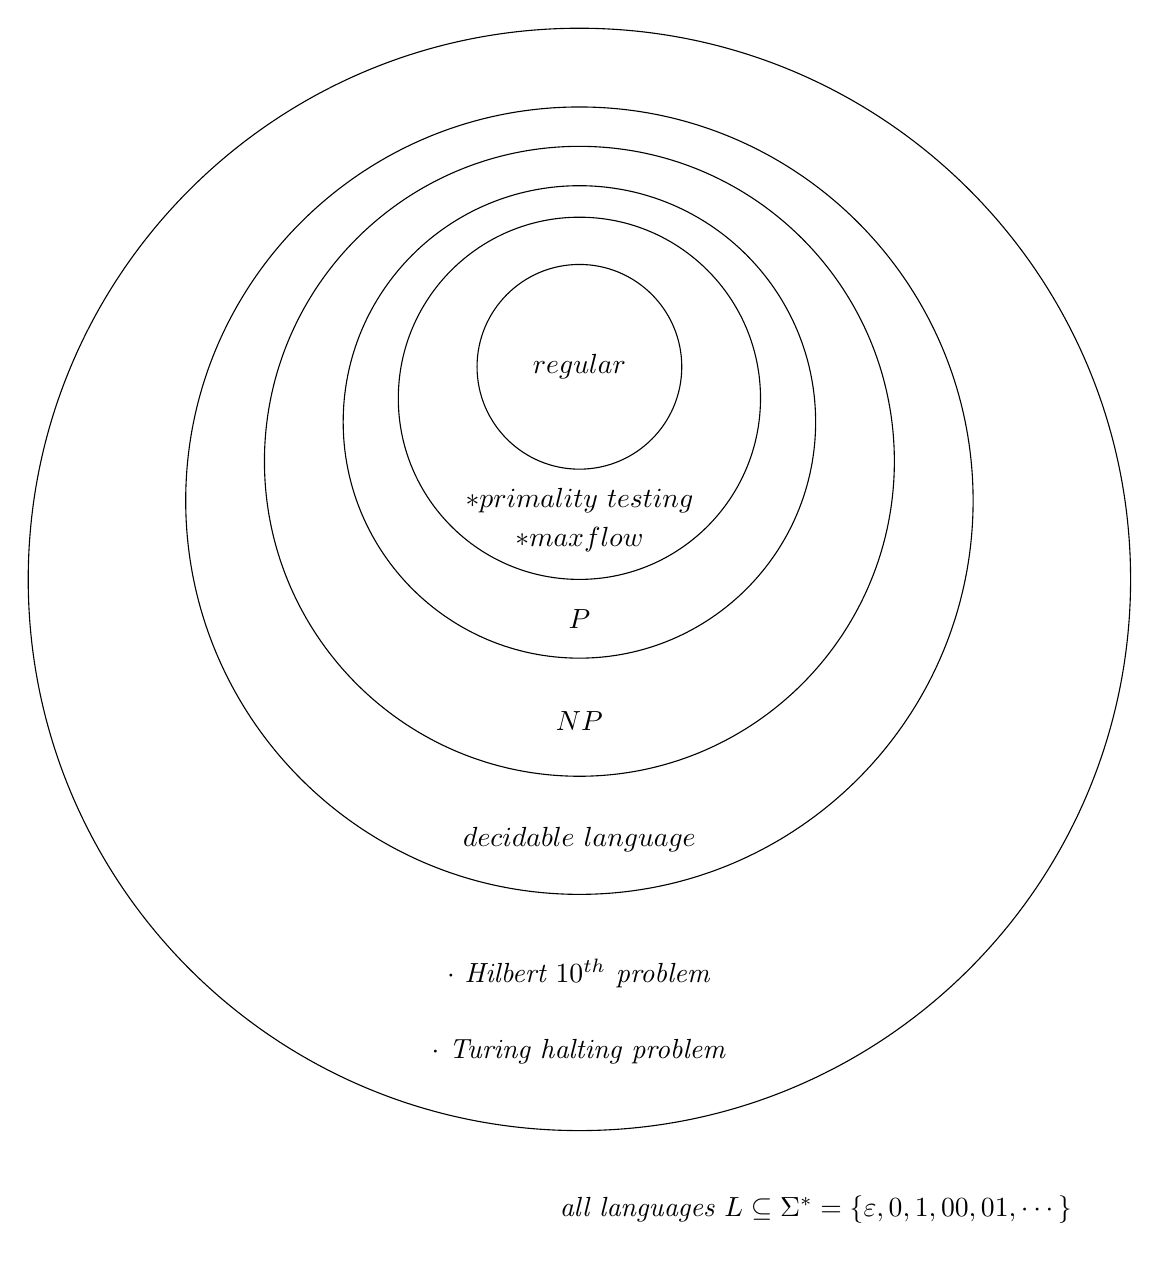
\begin{tikzpicture}
    % Draw circle
    \draw (0,0) circle (7cm);
    \draw (0,1) circle (5cm);
    \draw (0,1.5) circle (4cm);
    \draw (0,2) circle (3cm);
    \draw (0,2.3) circle (2.3cm);
    \draw (0,2.7) circle (1.3cm);

    % Add text
    \node at (0,2.7) {$regular$};
    \node at (0,1) {$*primality~testing$};
    \node at (0,0.5) {$*maxflow$};
    \node at (0,-0.5) {$P$};
    \node at (0,-1.8) {$NP$};
    \node at (0,-3.3) {$decidable ~ language$};
    \node at (0,-5) {\textit{$\cdot$ Hilbert $10^{th}$ problem}};
    \node at (0,-6) {\textit{$\cdot$ Turing halting problem}};
    \node at (3,-8) {\textit{all languages $L \subseteq \Sigma^* = \{\eps,0,1,00,01,\cdots\}$}};
\end{tikzpicture}

\begin{remark}
    \textit{\\\textbf{NP}: problems that are efficiently verifiable\\ \textbf{P}: problems that are efficiently solvable, i.e. solvable in $n^{O(1)}$ time\\\textbf{regular language}: problems that are solvable without memory, i.e. solvable by finite automation}
    
    \textit{number of regular languages: $\aleph_0$}

    \textit{number of all languages: $\aleph_1$}
\end{remark}

\ifx\allfiles\undefined
\end{document}
\fi